\documentclass[12pt,a4paper,twoside]{article}
\usepackage{graphicx}
\graphicspath{{figures/}}
\usepackage[margin=2.5cm]{geometry}
\renewcommand{\baselinestretch}{1.1}
\usepackage[english]{babel}
\usepackage[T1]{fontenc}
\usepackage[utf8]{inputenc}
\usepackage{siunitx}
\usepackage{amsmath}
\usepackage{ragged2e} %justify text
\numberwithin{equation}{section}
\usepackage{amsfonts}
\usepackage{amssymb}
\usepackage{braket}
\usepackage{cmap}
\usepackage{url}
\usepackage{caption}
\usepackage{subcaption}\usepackage{graphicx}
%\usepackage[usenames, dvipsnames]{color}
\usepackage{float}
\usepackage{xcolor}
\raggedbottom
\renewcommand\thesection{\arabic{section}}
\captionsetup{labelfont=bf,justification = justified,font=small}
%\usepackage[labelfont=bf,textfont=normalfont,singlelinecheck=off,justification=raggedright]{subcaption}
\usepackage[superscript,biblabel]{cite}
\usepackage{cancel}
\usepackage{adjustbox}
%Puts [] around citation number
\makeatletter \renewcommand{\@citess}[1]{\textsuperscript{\,[#1]}} %change reference style
%\usepackage{showframe} actually super useful
\usepackage[percent]{overpic}
\usepackage{mwe,tikz}
\usepackage{epstopdf}
\usepackage{enumitem}
\usepackage{verbatim}
\usepackage{relsize}
\renewcommand{\_}{\textscale{.7}{\textunderscore}}




\begin{document}

%\vspace{4cm}
\title{Template}


\author{\textbf{Lassi Linnala} \\ lassi.linnala.515@student.lu.se}


\maketitle



\vspace{1cm}

{Abstract Abstract Abstract Abstract Abstract Abstract}

\thispagestyle{empty}
\newpage
\pagenumbering{roman}

\newpage 
\tableofcontents
\clearpage
\pagenumbering{arabic}
\setcounter{page}{1}


\section{Introduction} 
The electronic band structure of graphene consists of Dirac cones as illustrated in Fig. \ref{dirac-cone-gr}. These Dirac cones are famous for their linear dispersion which results that the electron occupying these bands have zero effective mass.
\begin{figure}[H]
	\centering
	\begin{subfigure}{0.6\linewidth}
		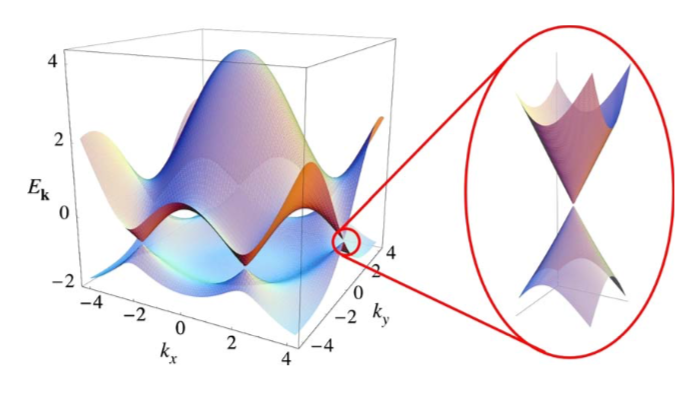
\includegraphics[width=1.0\linewidth]{Gr-dirac-cone.png}
	\end{subfigure}
	\caption{Electronic band structure and a Dirac cone of graphene. From {\cite{Castro-Neto}}.}
	\label{dirac-cone-gr}
\end{figure} 

\section{Method}

\subsection{Density functional theory}
The theoretical framework of DFT is based on the theorems by Hohenberg and Kohn\cite{Hohenberg-Kohn}. These theorems prove that the external potential is uniquely determined by the electron density, and that there exists an universal density functional in terms of which the total energy can be described. The density that minimizes this total energy is the true ground state density corresponding to the true ground state total energy. 

\begin{comment}
These theorems are remarkable in the sense, that by knowing the universal functional and the ground state density, the entire Hamiltonian could be constructed and all the properties of the system, both ground and excited, could be determined.
\end{comment}

While these theorems circumvent the otherwise impossible task of characterizing the many-body wave function by introducing the density. Hohenberg and Kohn did not manage to give an accurate description for the universal density functional. In particular, it has been difficult to formulate the many-body kinetic energy as a functional of density.

Kohn and Sham (KS) replaced the problem of finding the ground state density of the interacting system with an auxiliary non-interacting system, under the assumption that the ground state densities of the non-interacting and the interacting systems are equal\cite{Kohn-Sham}. The genius of this proposal was that the kinetic energy could now be determined from the one-particle orbitals $\phi_i(\textbf{r})$ of the non-interacting system, 
\begin{comment}
\begin{equation}
    T_0[\rho] = -\frac{1}{2}\sum_{i}^{N}\int dr \phi_i^*(r)\nabla^2\phi_i(r).
\end{equation}
\end{comment}
\begin{equation}
    T_0[\rho] = -\sum_{i}^{N/2}\int d^3r \phi_i^*(\textbf{r})\nabla^2\phi_i(\textbf{r}), 
\end{equation}
where it has been assumed that the system is non-magnetic such that each of the $N/2$ orbitals is occupied twice.

In terms of this non-interacting kinetic energy, the KS total energy of the interacting many-body system is,
\begin{equation}\label{KS:total-energy-functional}
    E_{\textrm{KS}}[\rho] = T_0[\rho] + E_{\textrm{H}}[\rho] + E_{\textrm{XC}}^{\textrm{DFT}}[\rho] + \int d^3r v_{\textrm{ext}}(\textbf{r}) \rho(\textbf{r}),
\end{equation}
where $E_{\textrm{H}}$ is the Hartree term describing the Coulomb interaction of two charge densities,
\begin{equation}\label{eq:Hartree-energy}
    E_{\textrm{H}}[\rho] = \frac{1}{2}\int d^3r d^3r' \frac{\rho(\textbf{r}) \rho(\textbf{r}')}{|\textbf{r}-\textbf{r}'|},
\end{equation}
and $E_{\textrm{XC}}^{\textrm{DFT}}[\rho]$ is the XC functional of DFT.
\begin{comment}
, and in DFT we can further note that this term should also account, in theory, for the fact that the kinetic energy is of the non-interacting KS system. \textcolor{red}{Need write better?}
\end{comment}

The density which minimizes the KS total energy is also evaluated from the (doubly occupied) one-particle orbitals of the non-interacting system, 
\begin{equation}
    \rho(\textbf{r}) = 2\sum_{i}^{N/2} |\phi_i(\textbf{r})|^2. 
\end{equation}
These orbitals are given by solving the KS equations,
\begin{equation}\label{eq:Kohn-Sham-equations}
    \bigg[-\frac{1}{2}\nabla + V_{\textrm{KS}}(\textbf{r})\bigg] \phi_i(\textbf{r}) = \varepsilon_i\phi_i(\textbf{r}),
\end{equation}
where the electron in the non-interacting system feels the effective KS potential,
\begin{equation}\label{eq:Kohn-sham-potential}
    V_{\textrm{KS}}(\textbf{r}) =  \int d^3r' \frac{\rho(\textbf{r}')}{|\textbf{r}-\textbf{r}'|} + \frac{\delta E_{\textrm{XC}}^{\textrm{DFT}}[\rho]}{\delta\rho(\textbf{r})} + v_{\textrm{ext}}(\textbf{r}).
\end{equation}

\begin{comment}
This potential is given by taking the functional derivatives of the terms in the KS total energy, excluding the kinetic energy, with respect to the density $\rho(\textbf{r})$. 
\end{comment}

These equations are then solved self-consistently. Starting from an initial guess of the density, KS potential can be constructed. Solutions of the KS equations then give a new density, which can be used to calculate the KS total energy and related properties of the interacting many-body system. For this new density, a new KS potential can be constructed and the KS equations can again be solved for a new density. This is repeated until the change in a parameter, such as the total energy, between two concurrent loops is smaller than an user defined convergence parameter. Reaching this convergence then gives the ground state energy and density of the interacting many-body system, based on which various properties can be derived.

\section{Results and Discussion}
this is the results section, where I have tested figure font sizes
\begin{figure}[H]
	\centering
	\begin{subfigure}{0.31\linewidth}
		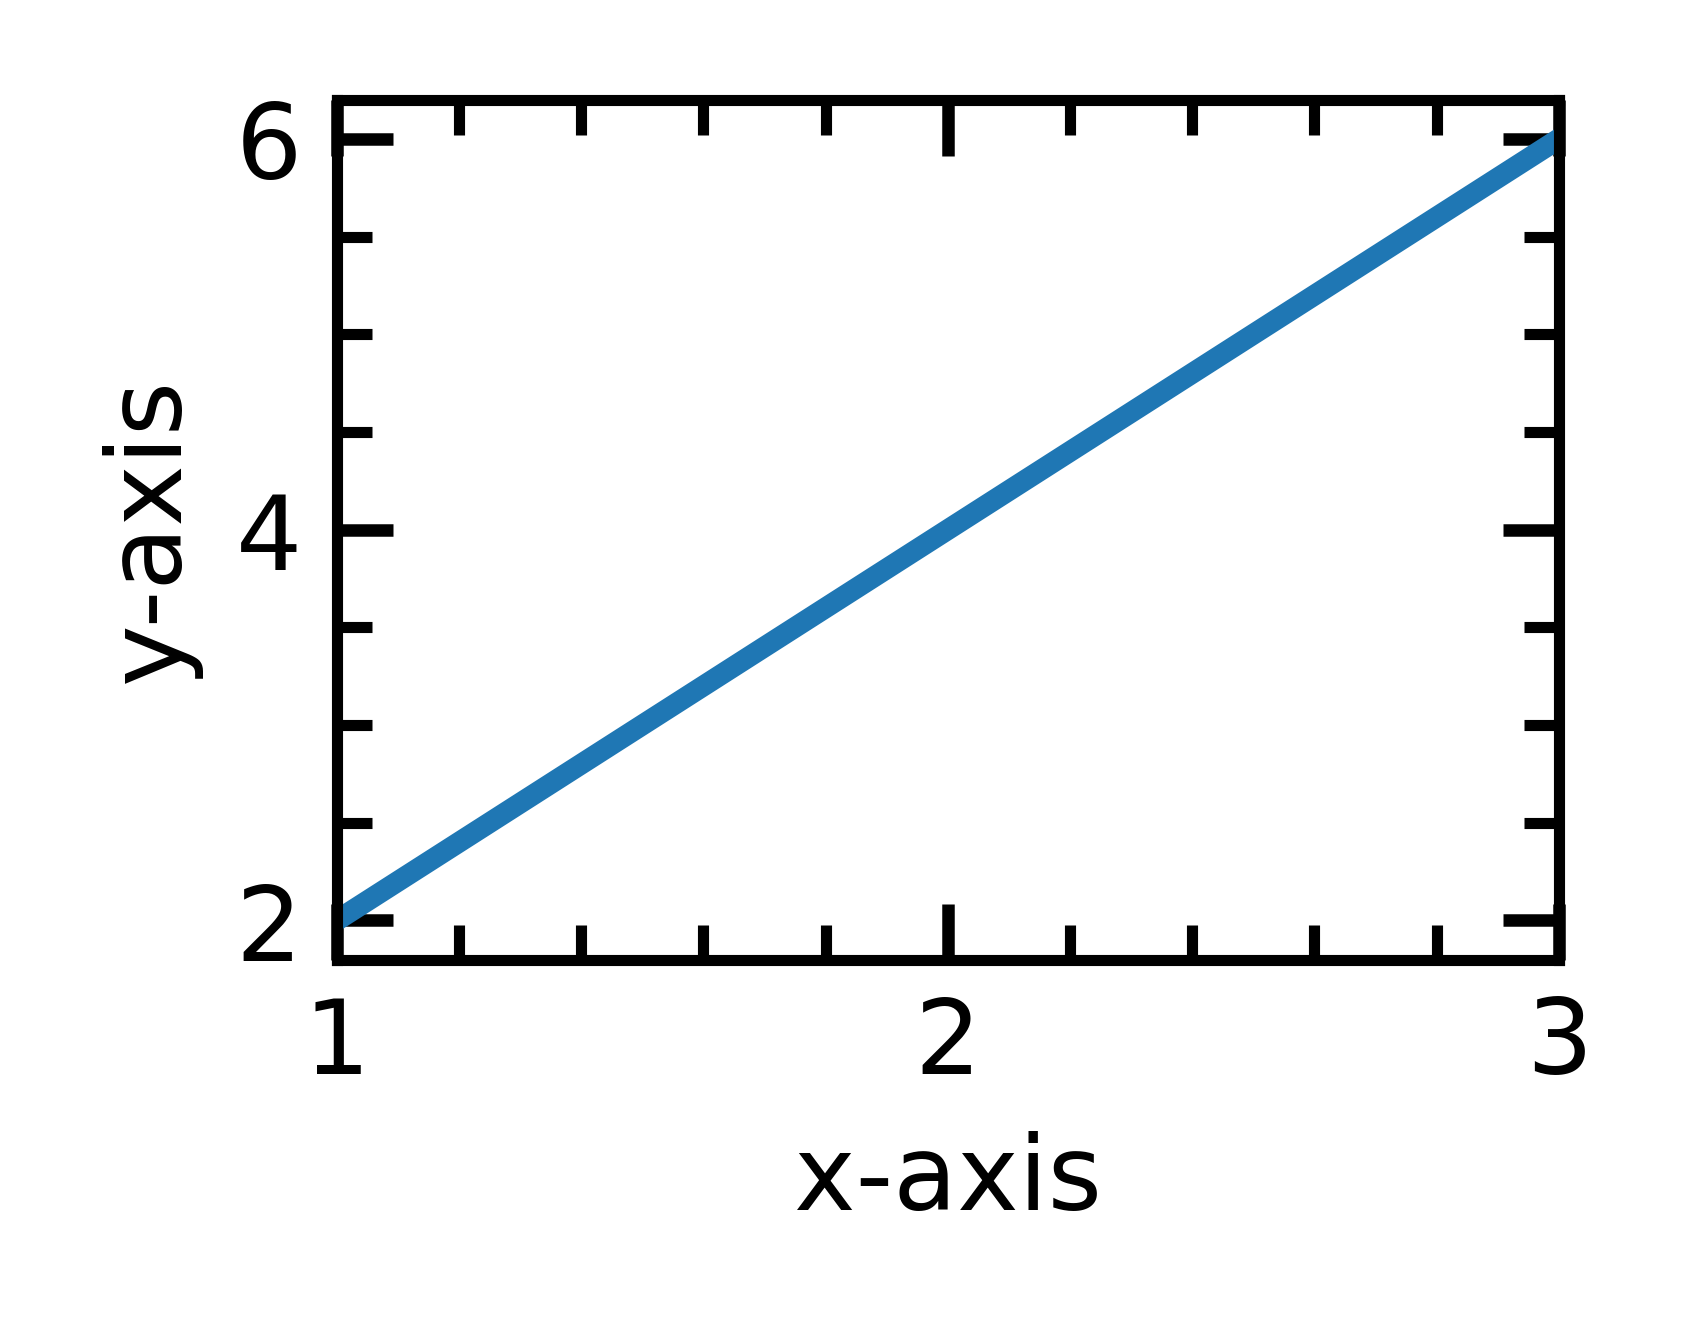
\includegraphics[width=1.0\linewidth]{3x3.png}
	\end{subfigure}
    \begin{subfigure}{0.31\linewidth}
		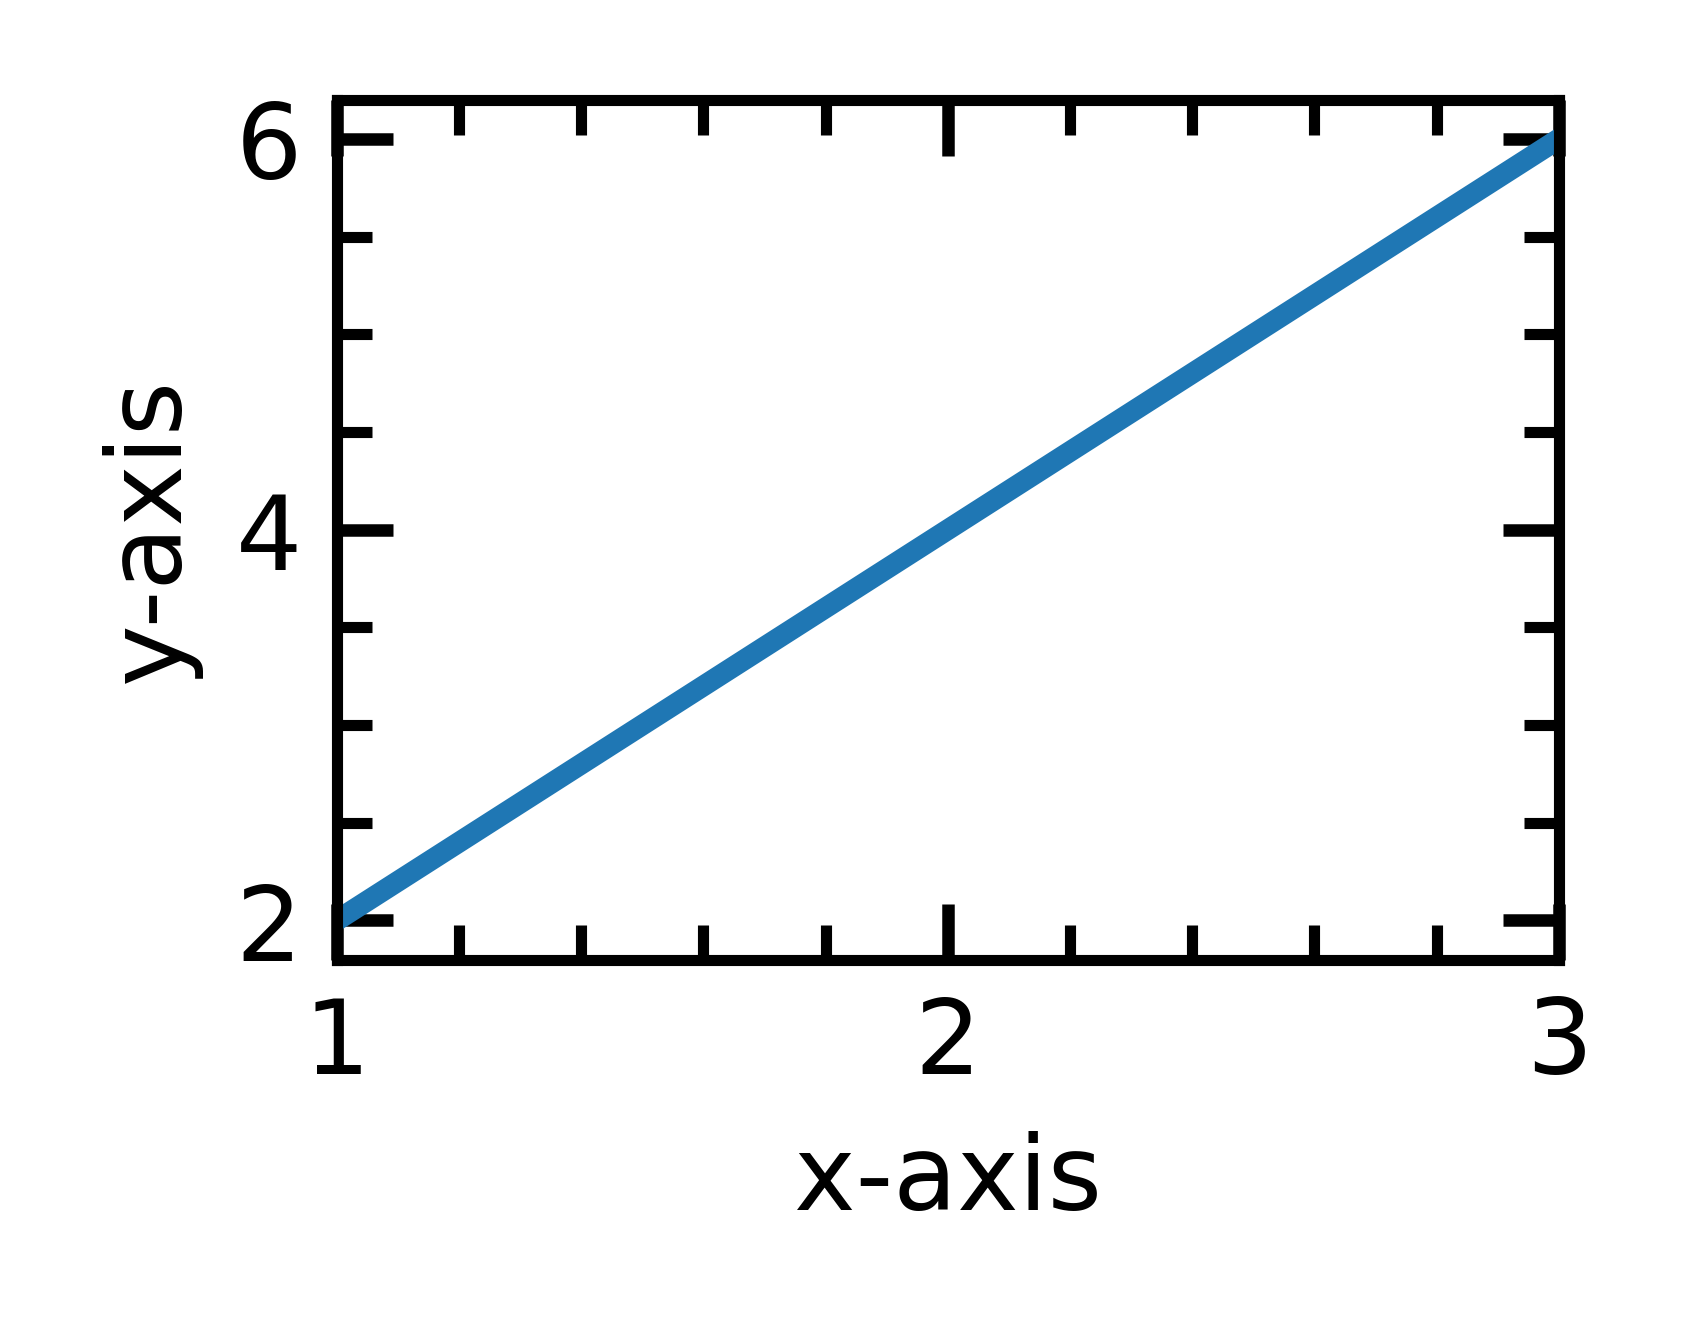
\includegraphics[width=1.0\linewidth]{3x3.png}
	\end{subfigure}
    \begin{subfigure}{0.31\linewidth}
		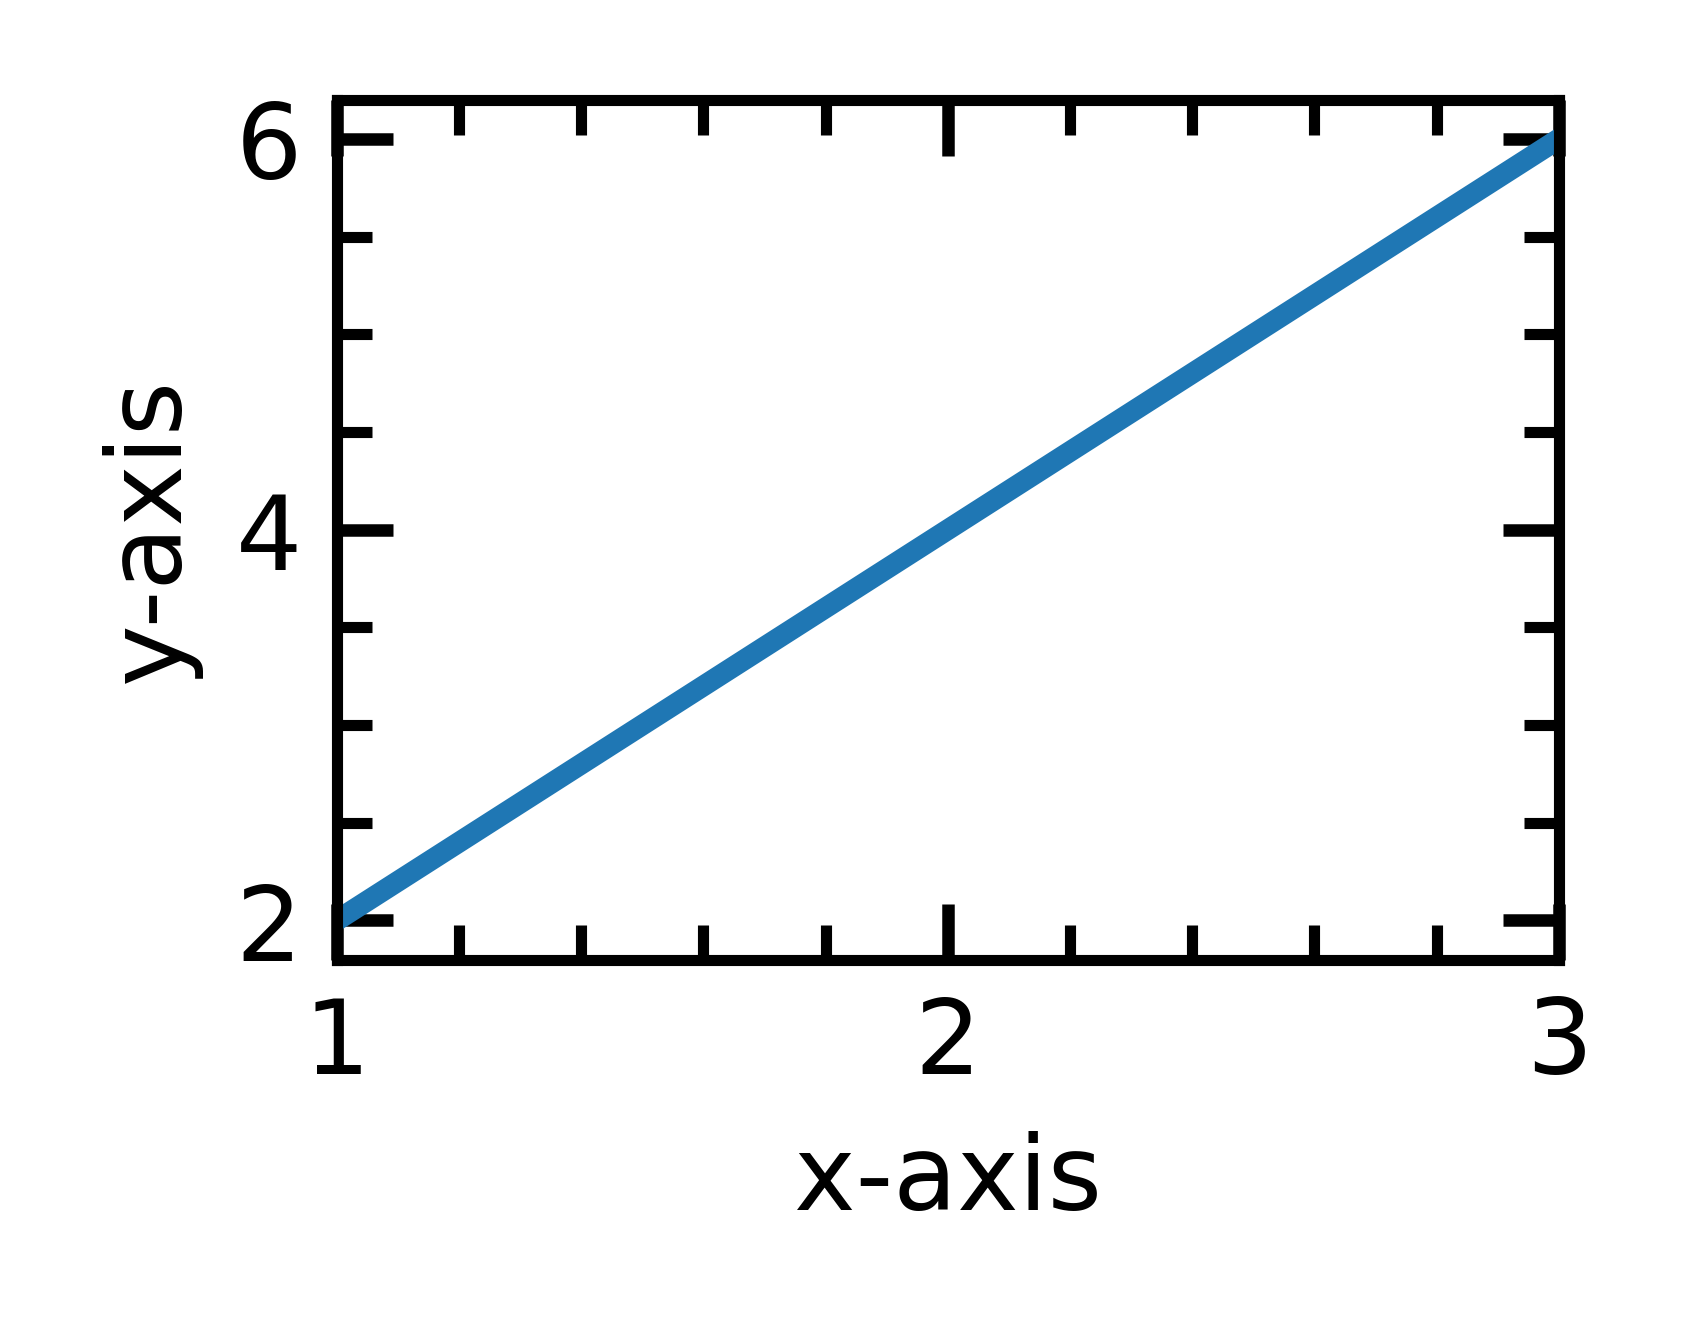
\includegraphics[width=1.0\linewidth]{3x3.png}
	\end{subfigure}
    \caption{Test 3x3 figures.}
\end{figure} 

\begin{figure}[H]
	\centering
	\begin{subfigure}{0.48\linewidth}
		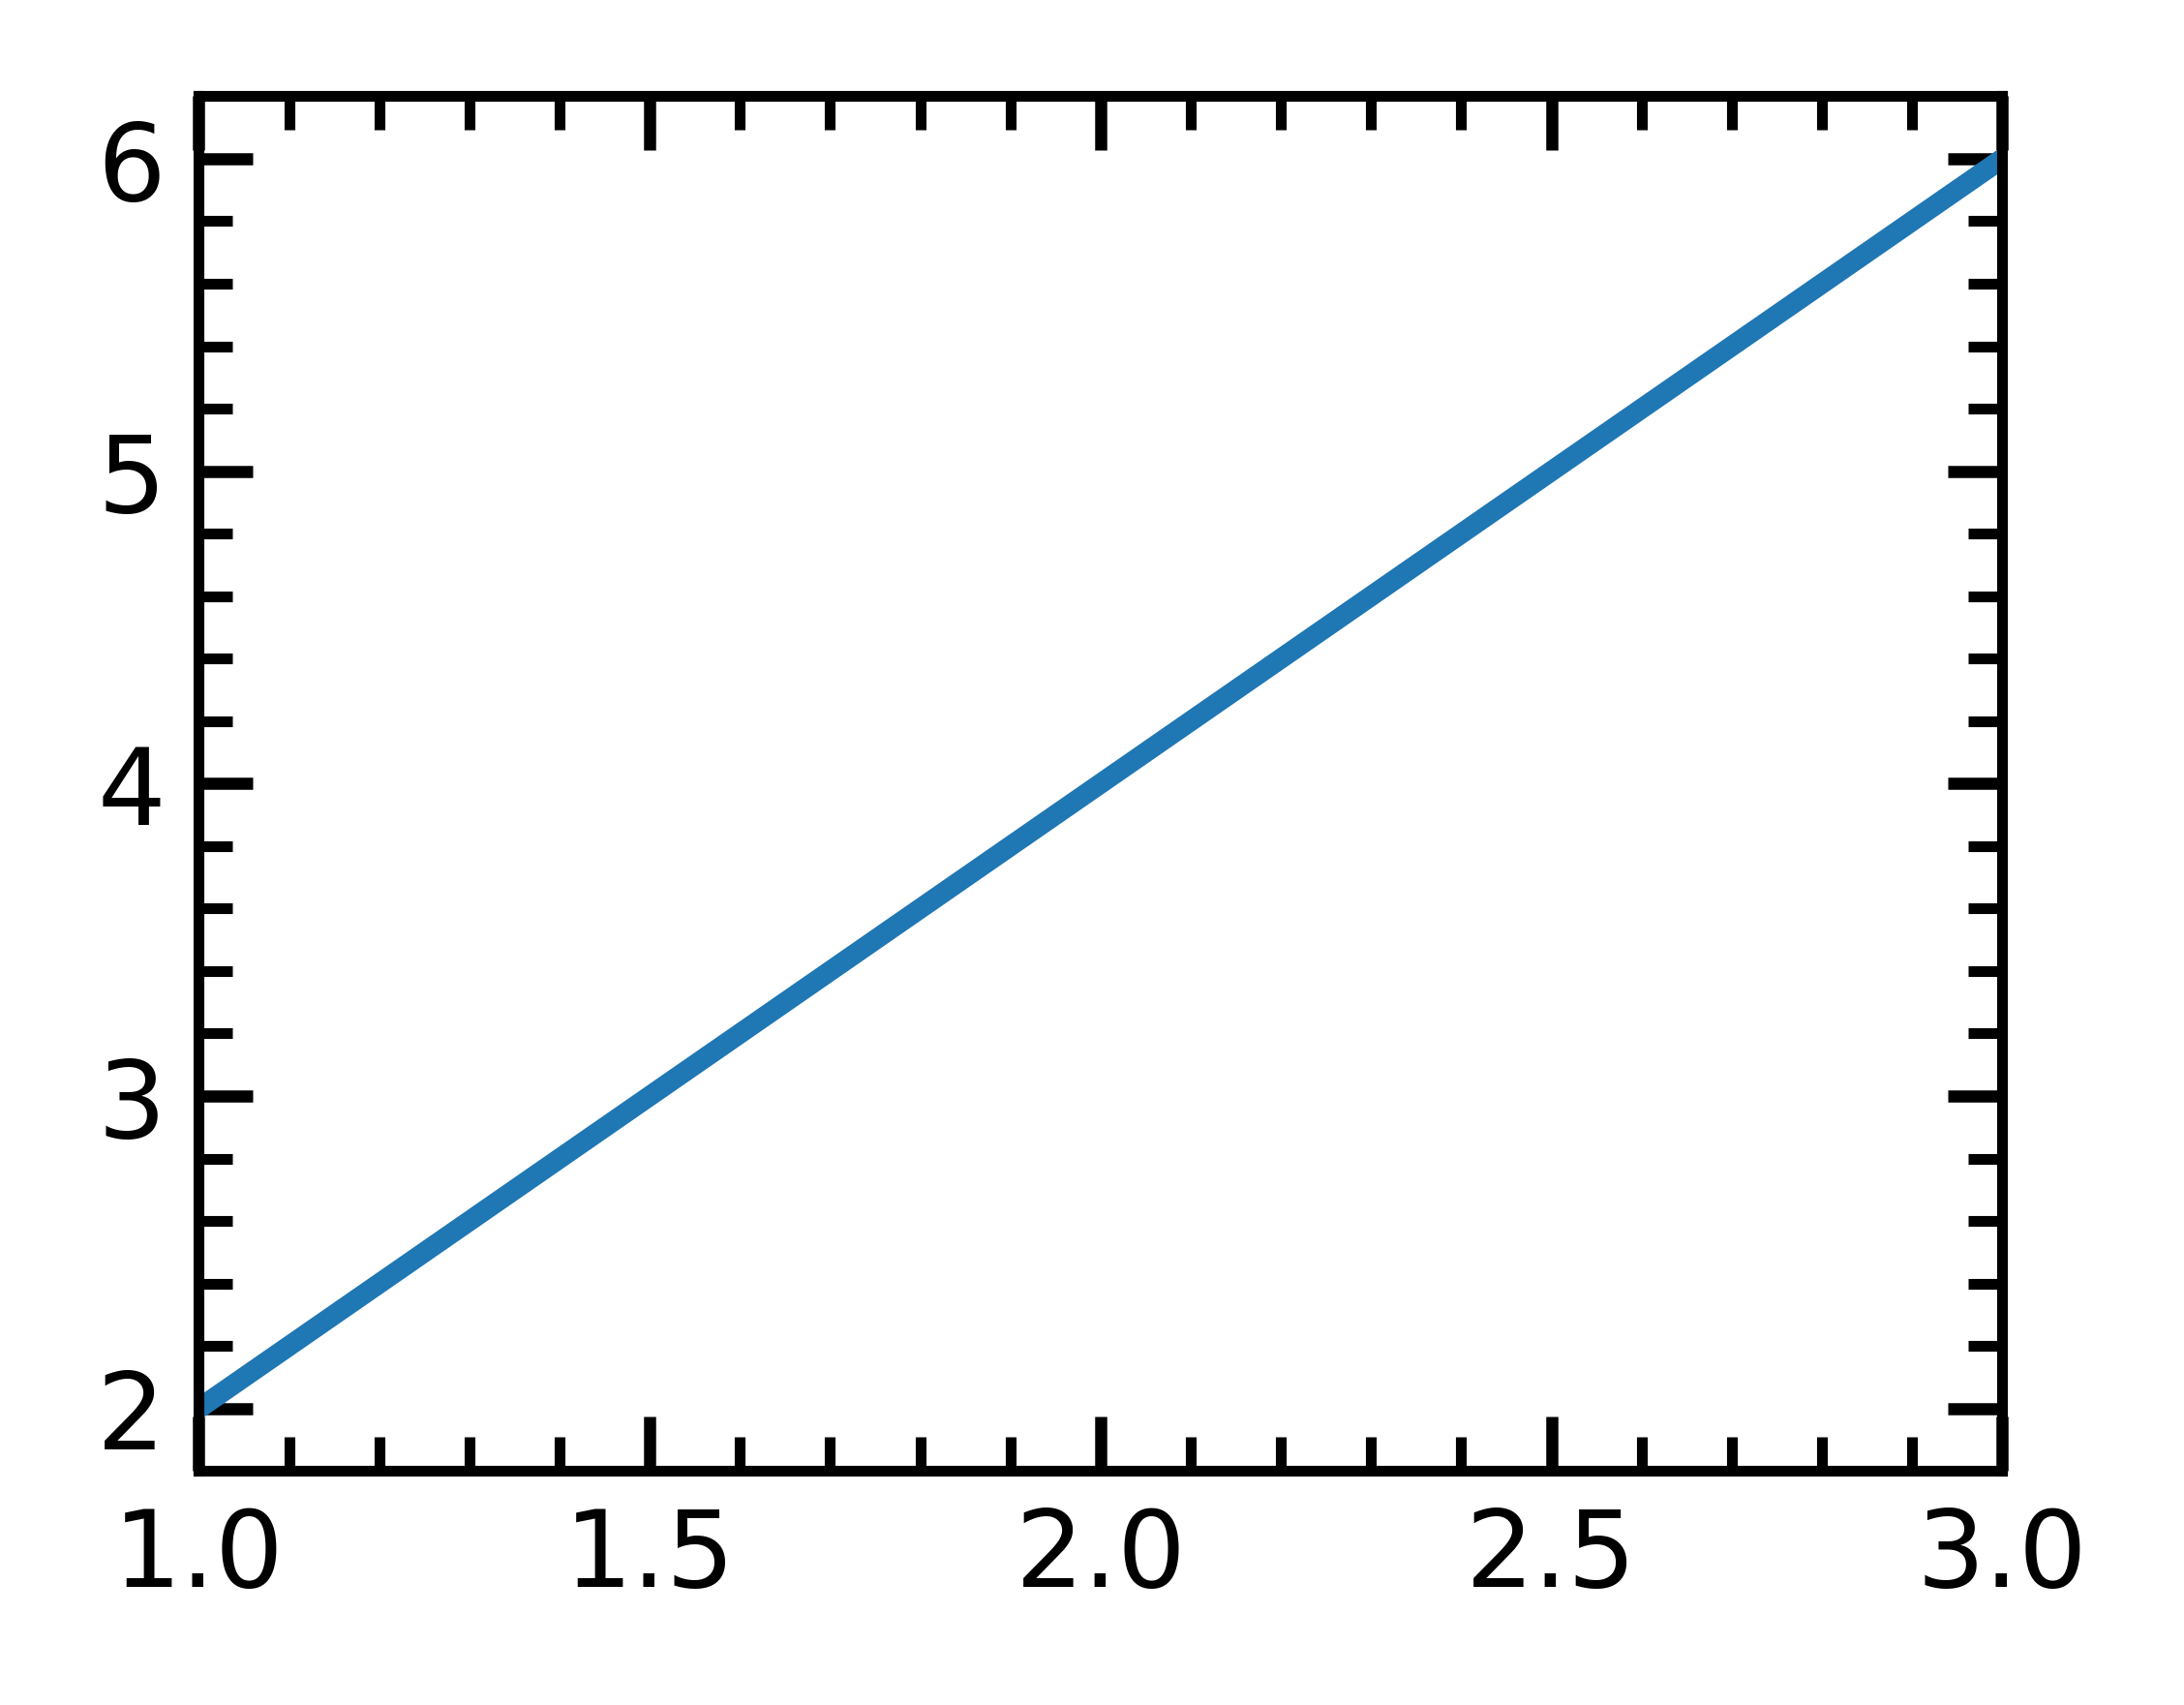
\includegraphics[width=1.0\linewidth]{2x2.png}
	\end{subfigure}
    \begin{subfigure}{0.48\linewidth}
		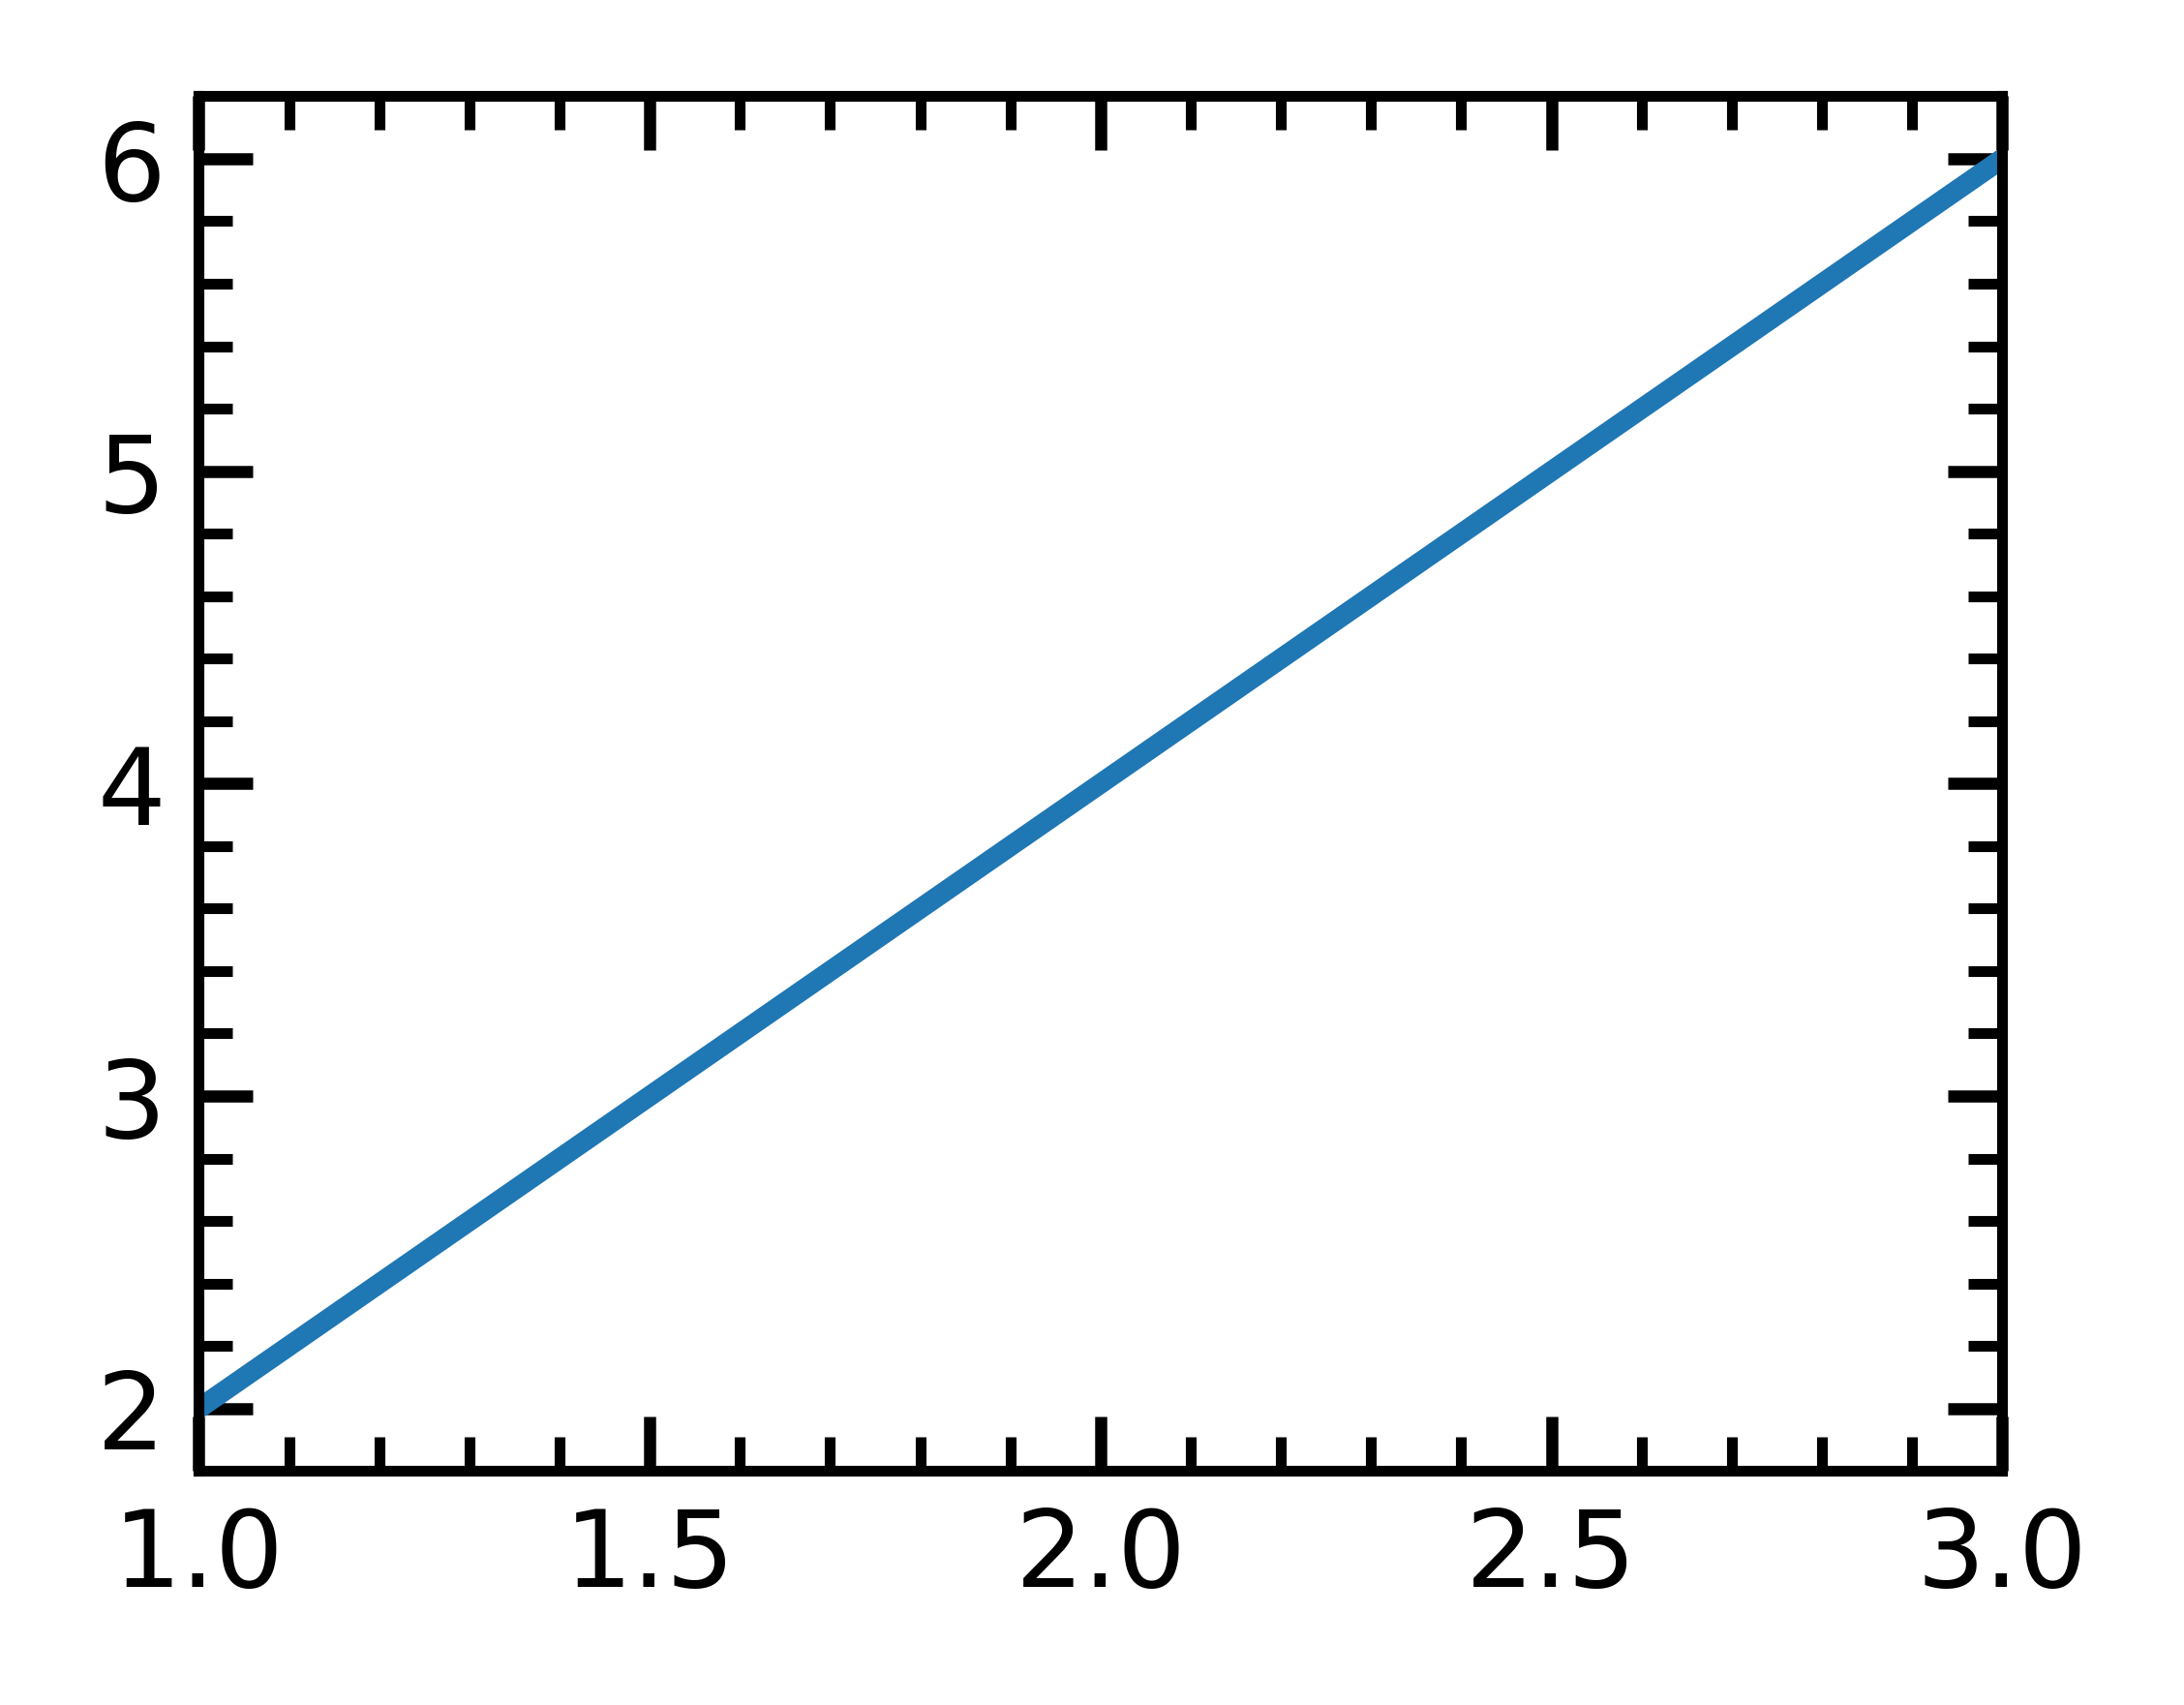
\includegraphics[width=1.0\linewidth]{2x2.png}
	\end{subfigure}
    \caption{Test 2x2 figures.}
\end{figure} 

\begin{figure}[H]
	\centering
	\begin{subfigure}{0.65\linewidth}
		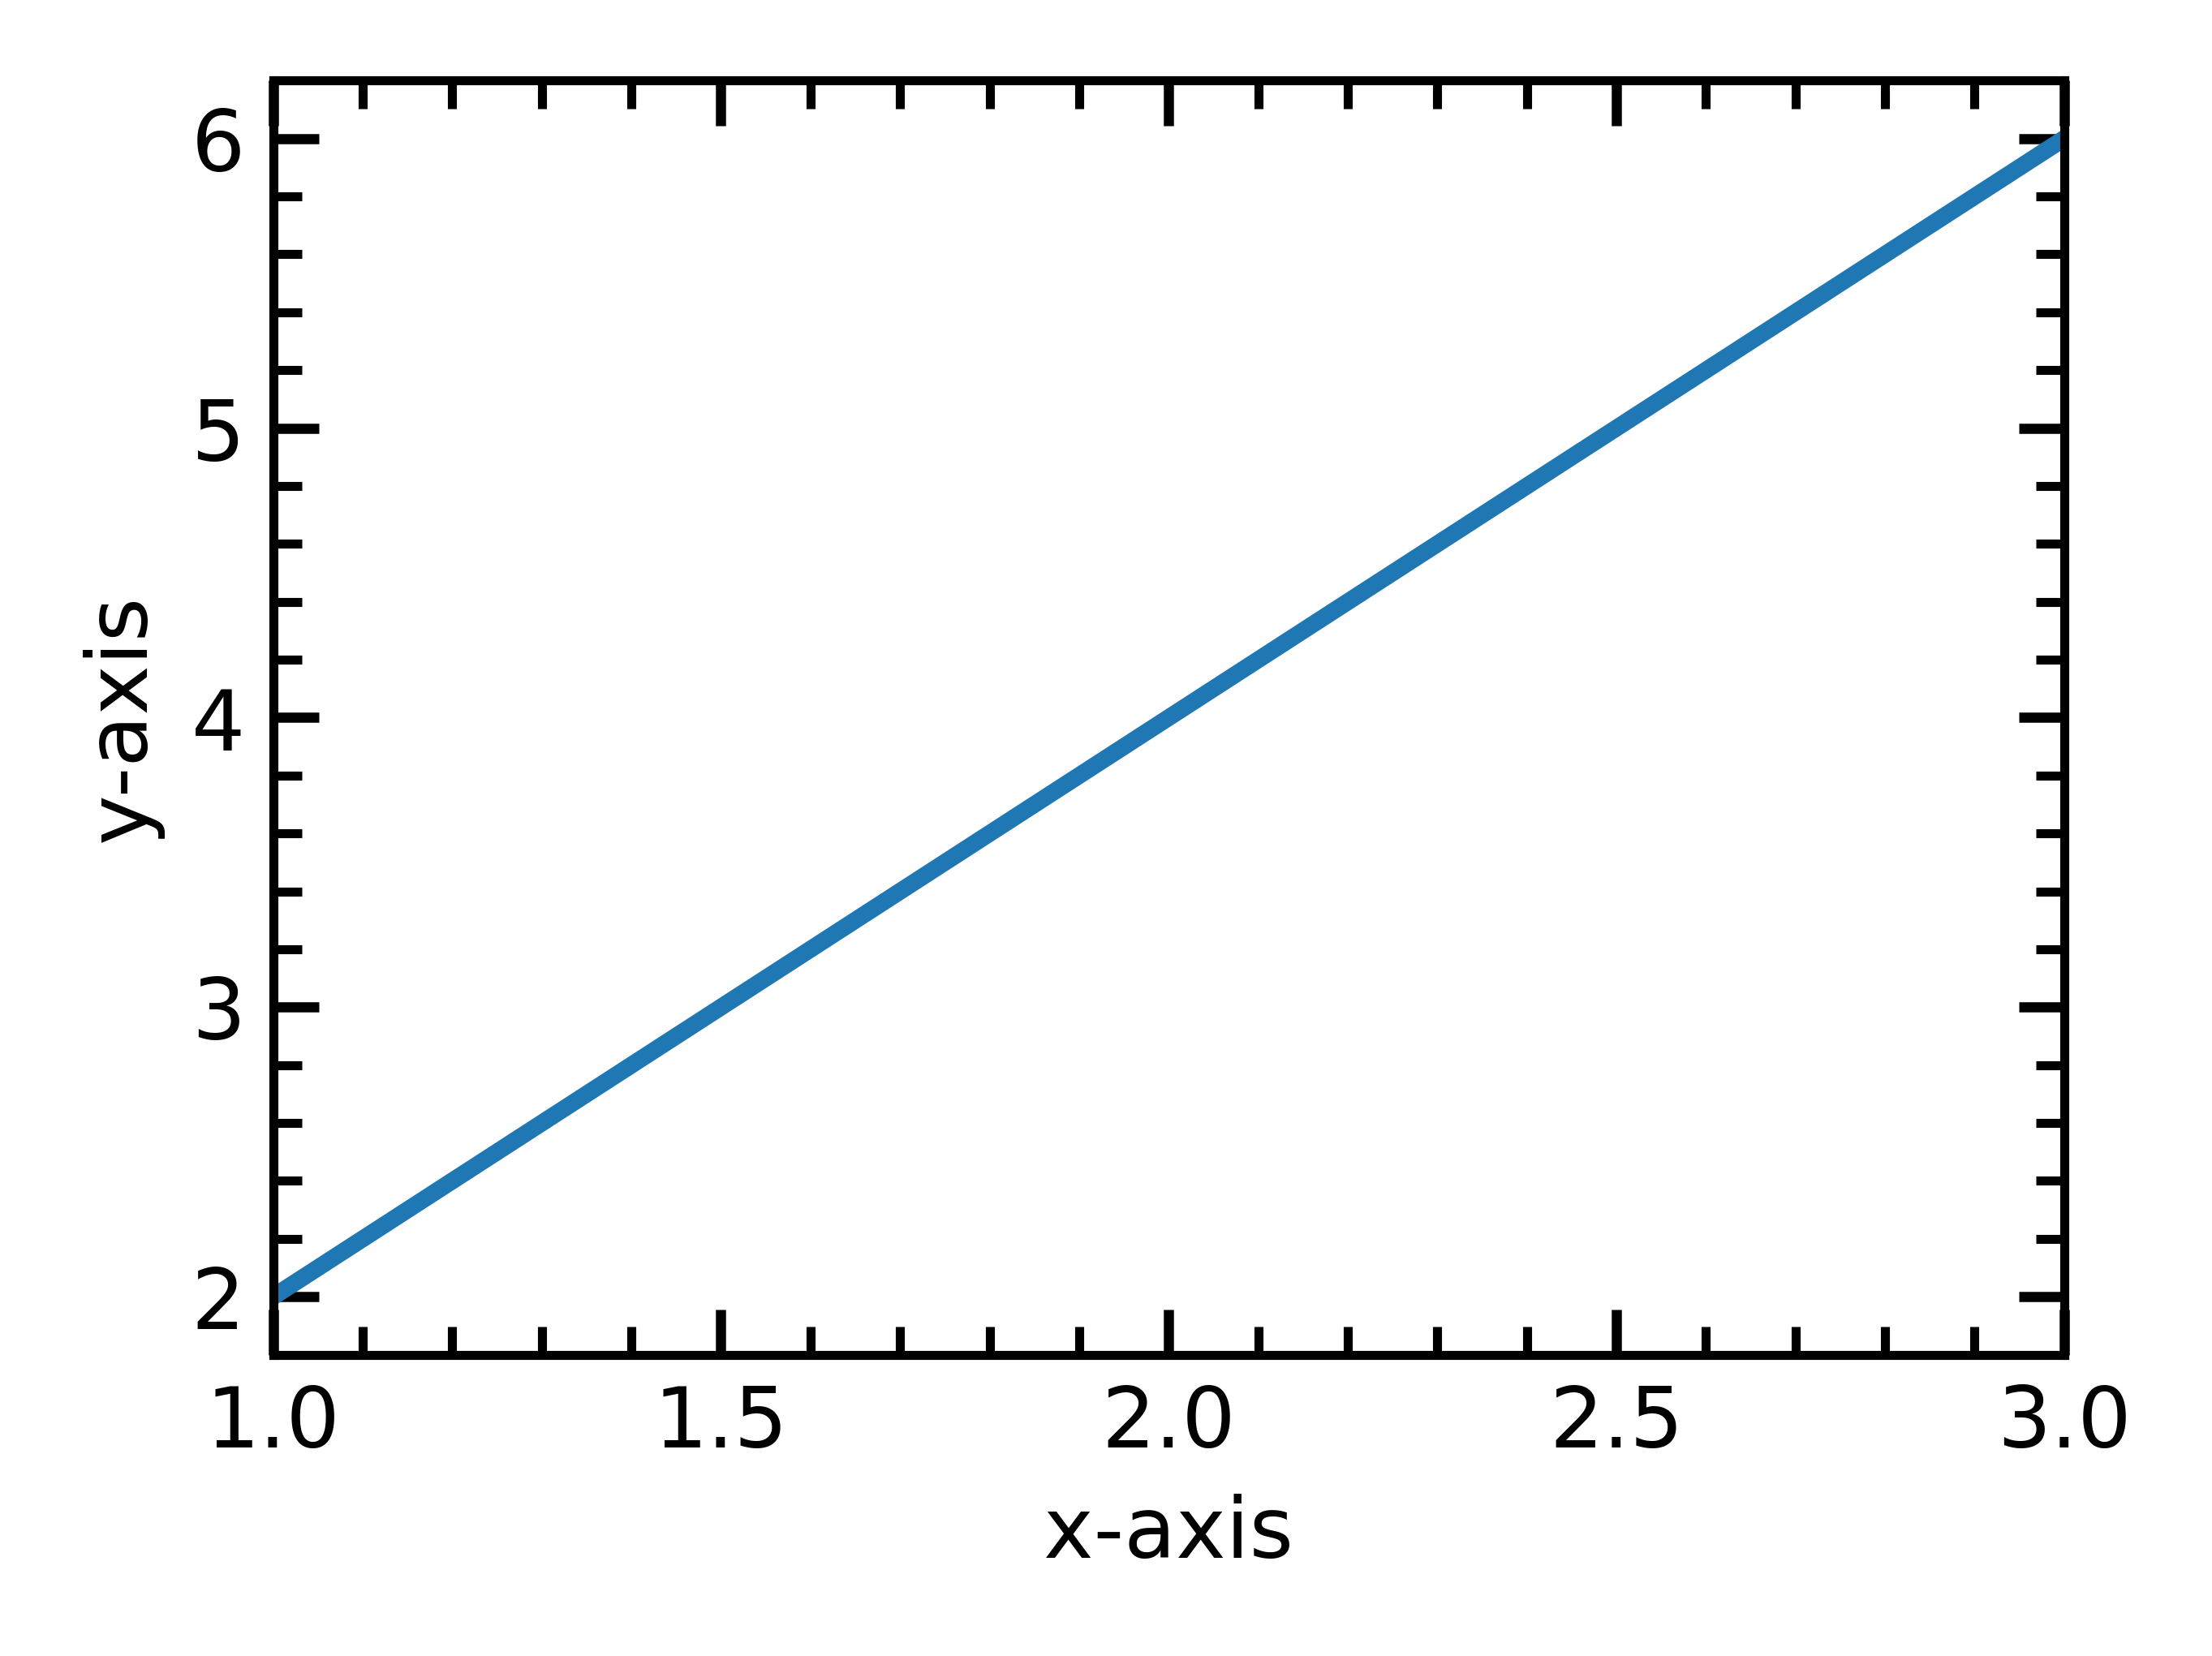
\includegraphics[width=1.0\linewidth]{1x1.png}
	\end{subfigure}
    \caption{Test 1x1 figures.}
\end{figure} 

\begin{table}[H]
  \begin{center}
   \caption{Character table of the point group $T_d$ in the Mulliken notation and the decomposition of the phonon rep for zincblende InSb.}\label{table:Td_character-main-text}
    \begin{tabular}{ | c | c  c  c  c  c | c  |}
      \hline
      $T_d$ & $e$ & $8C_3$ & $3C_2$ & $6S_4$ & $6\sigma_d$ &      \\ \hline

      $\textrm{A}_1$ & $1$ & $1$ & $1$ & $1$ & $1$ &  \\ 
      
      $\textrm{A}_2$ & $1$ & $1$ & $1$ & $-1$ & $-1$ & \\
      
      $\textrm{E}$ & $2$ & $-1$ & $2$ & $0$ & $0$ &  \\
      
      $\textrm{T}_1$ & $3$ & $0$ & $-1$ & $1$ & $-1$  &\\
      
      $\textrm{T}_2$ & $3$ & $0$ & $-1$ & $-1$ & $1$ & $(x,y,z)$, $(xy,yz,xz)$ \\ \hline
      
      $\chi^{\textrm{InSb}}$ & $6$ & $0$ & $-2$ & $-2$ & $2$ & $\chi = \sum_{\alpha} m_{\alpha} \chi^{\alpha}$ =   $2\textrm{T}_2$ \\ \hline
    \end{tabular}
  \end{center}
\end{table}

\section{Conclusion}
Conclusion


%%%%------ END OF THE DOCUMENT ------%%%%
\newpage 
%\pagenumbering{} %page number or not
\flushleft

\addcontentsline{toc}{section}{References}
\bibliography{References}
\bibliographystyle{ieeetr}

%%%%%%%%%APPENDICES%%%%%%%%%

\newpage

\section*{Appendices}
\addcontentsline{toc}{section}{Appendices}

\subsection*{A \hspace{5pt} Appendix}
\addcontentsline{toc}{subsection}{A Appendix}
\justifying


\end{document}





